    
        \subsection{Problem Statement}
        In this part of the problem we are asked to "create a model that predicts whether an individual worker whose job is remote-ready will be allowed to and will choose to work from home".\\ \\ We take this to mean "given the characteristics of an individual worker such as their age, income, and family status, determine the probability that a worker with these characteristics will be allowed to \textit{and} want to from home, versus in the office. Then, compare this probability to a threshold value to give the binary answer of yes the worker will work from home or no they won't." \\ \\ This problem definition is advantageous because it scales more easily to larger numbers of people with the same characteristics, which will be needed when this model is reused in Q3. As human choices are not deterministic, a level of stochasticity can be employed if we use the probabilities, meaning not everyone with the same characteristics behaves in the same way.

        \subsection{Assumptions and Justifications}
            \begin{enumerate}[label={2.\arabic*.}]
                % All assumptions made in the model must be stated and justified. Do this in the following way:
                % \item creates a new bullet point for the new assumption
                % \assume{The thing you are assuming}{The justification for this assumption}
                % So overall write this: \item \assume{assumption}{justification}
                \item \label{independence} \assume{Whether a worker wants to work from home can be treated as independent of whether they are allowed to, and are in a remote ready job.}{This is a logical assumption because it is plausible to want to work from home but not be allowed to, to want to work from home and be allowed to, to not want to work from home and not be allowed to, and to not want to work from home and not be allowed to. In a purely theoretical sense, workers can make a decision on what they want to do separately from what they are allowed to do.}
                \item \label{representative} \assume{2019 ONS Data \cite{ONS2} for the proportion of workers of different ethnicities, sexes, professions etc. is representative of the pre-pandemic probability that a worker of the given ethnicity/sex etc. will work from home.}{The data was collected with a large sample size by a substantial public statistics organisation so it is reasonable to suppose this is the case. We use the most recent pre-pandemic data as this is likely to be the most representative.}
                \item \assume{We can account for the impact of the pandemic on working from home by applying a pandemic constant correction factor.}{This reflects how attitudes have changed toward remote working over the course of the pandemic. It would be preferred to determine this on the level of an individual but this requires data we don't currently have access to. See Extending the Model}
                \item \assume{The maximum age of a working person is 80 years and the minimum age is 20 years.}{This is probably an overestimate but should definitely not be an underestimate, which is important for our model to avoid negative age multipliers.}
                \item \assume{Working age is (apart from the above constraints), normally distributed with mean 35 and standard deviation 10}{This is likely because we would expect ages to be roughly symmetrical as there are factors which would both prevent younger workers getting into the labour market (education) and remove older workers (retirement). As we don't know the distribution and in the interests of time we make this assumption. By the 68–95–99.7 rule these parameter choices give us 99.7\% of the data within the stated min/max, meaning artificially rounding values into this range has next to no effect.} 
            \end{enumerate}
      
             
        \subsection{Analysing the Problem}  \label{analysis}
           It is insightful to represent the problem in probability notation.
            For a given worker, we define the following events.
            \begin{itemize}
                \item $W$, the event that the worker wants to work from home.
                \item $R$, the event that the worker's job enables them to work from home (remote ready job).
                \item $A$, the event that the worker's employer allows them to work from home. 
                \item $W_p$, the event that the worker wants to work from home pre-pandemic.
            \end{itemize}           
            We also define a pandemic correction $c$ for the worker which is a multiplying factor so that:
            \begin{equation}
                P(W) = \min{(1,c \cdot P(W_p))}
            \end{equation}
            This is designed to reflect how the pandemic has changed attitudes towards remote working. 
            
            With these events, what the question is asking for becomes clear:
            \begin{equation}
                P((W \cap A) | R) \equiv \frac{P(W \cap A \cap R)}{P(R)}
            \end{equation}
           \textit{To simplify the notation we omit conditioning on all of the features of the worker, as we can determine the probabilities of events derived from W, A, R from the worker's features.}\\
           
           Under Assumption \ref{independence} we can perform the following manipulation:
            \begin{equation}
                P((W \cap A) | R) \equiv \frac{P(W)\cdot P(A \cap R)}{P(R)} \equiv  \frac{c\cdot P(W_p)\cdot P(A \cap R)}{P(R)} \equiv  \frac{c\cdot P(W_p \cap A \cap R)}{P(R)}
            \end{equation}           
            
        \subsection{Defining Variables \& Constant Parameters} % To use an & or % you must put a \ before it or it is interpreted as a command.
            \subsubsection{Identifying Factors which affect the Outcome}
                %Explain here which variables/constants you thought were important when modelling this part of the problem and why they are important, how you came about identifying them and their values, and which ones you discarded or didn't include and why.
                % Detailed description of them and justification for why they are included (can use bps - itemize)
                
                When it comes to determining which workers work from home, the following factors were considered to be important. These were then condensed into variables for the model below.
                
                \begin{itemize}
                    \item \assume{Age}{The age of a worker will affect how "tech-savvy" they are, and remote working requires advanced use of digital technology, and also it will affect how much of an active social life the worker has.}
                    \item \assume{Commute Time}{In \cite{ONS}, the authors determine that "work-life balance was the greatest positive" of home working, and time spent commuting is reduced by home working, which affects work-life balance.}
                    \item \assume{House Features}{Working from home is dependent on whether or not a given worker has the space at home to concentrate and work.}
                    \item \assume{Income}{Working from home requires less transport costs which saves money, but infrastructure such as a good broadband connection is required.}
                    \item \assume{Sex}{This may affect the activities the way in which the person socialises with work colleagues, which could be an incentive to come into the office.}
                    \item \assume{Industry}{This affects their potential productivity when working from home, which may decide whether they are allowed to work from home.}
                    
                \end{itemize}
                
                The following features were discounted for the given reasons:
                \begin{itemize}
                    \item \assume{Family Characteristics}{Workers with young children may need to work from home to look after them, or alternatively may be distracted by them and want to work in the office. It was deemed not worth the time to investigate which of these is most likely. It can also be argued that the worker should not have to see their children if they are working from home; they may use a childminder.}   
                    \item \assume{Income}{Unfortunately we didn't have the required data to perform the below analysis for income as well as the factors used.}
                    \item \assume{Size of Team - how many others are working from home?}{It is important to maintain a workplace culture so for large organisations some staff may be required to come into the office, while for small businesses working from home may be preferred to cut costs. However the data was not available so this feature had to be discarded}
                \end{itemize}                
                
            \subsubsection{Table of Variables/Constants}
                % To summarise all of the choices made.
                % All tables should have a title, a header, a label, and a caption.
                \begin{table}[H]
                  \begin{center}
                    \label{tab:variables2} % Use this to create a label for the table so you can later reference it with \ref
                    \begin{tabular}{|c|c|p{6cm}|p{6cm}|c|} % Defines where vertical lines appear and the column alignment left centre or right
                      \toprule 
                       \textbf{Type} & \textbf{Symbol} & \textbf{Definition} & \textbf{Value} & \textbf{Units} \\
                      \midrule 
                       Constant & \(\sigma\) & Age standard deviation & 10 & years  \\ % & used to separate cells in a row; \\ used to separate rows.
                      \midrule 
                       Constant & \(\mu\) & Age mean & 35 & years  \\ % & used to separate cells in a row; \\ used to separate rows.
                      \midrule 
                       Variable & \(A\) & Age of a given worker & $20 < A < 80$ & years  \\ % & used to separate cells in a row; \\ used to separate rows.
                      \midrule 
                       Variable & \(S\) & Sex of a given worker & Male/Female & years  \\ % & used to separate cells in a row; \\ used to separate rows.
                      \midrule 
                       Variable & \(E\) & Ethnicity of a given worker & White/Mixed/Black/Asian/Other & None  \\ % & used to separate cells in a row; \\ used to separate rows.
                      \midrule 
                       Variable & \(I\) & Industry in which a given worker works & Selected from the ONS Standard Industrial Classification (SIC) Grouping \cite{ONSGroup} & None  \\ % & used to separate cells in a row; \\ used to separate rows.
                      \midrule 
                       Variable & \(L\) & Level of education of a given worker & No Qualification, GCSE, A Level, etc. American and British qualifications converted to standardise as necessary. & None  \\ % & used to separate cells in a row; \\ used to separate rows.
                      \midrule 
                       Variable & \(T\) & Time a worker works & Part Time or Full time & None  \\ % & used to separate cells in a row; \\ used to separate rows.
                      \midrule 
                       Variable & \(C\) & Commute Length of a given worker & 0 to 10000 & m  \\ % & used to separate cells in a row; \\ used to separate rows. 
                      \midrule 
                       Variable & \(H\) & Whether their house allows work from home or not. i.e. do they have a quiet place to work, based on average house sizes in the region & True/False & None\\
                      \midrule 
                       Constant & \(c\) & Pandemic WFH attitudes correction. We choose this value because data from \cite{VOXEU} figure 3 suggests that (cancelling out the hugely improved and worsened reactions) the average tolerance of working from home increased by 40\% during the pandemic. & 1.4 & None\\
                      \bottomrule 
                    \end{tabular}
                    \caption{Summary of Problem 2 Variables \& Constant Parameters}                
                  \end{center}
                \end{table}
            
 
        \subsection{Developing the Model}  
            %Describe mathematical approaches and..
            %..Justify modelling used, including the use of technical computing. Why does it make sense?
            % Motivate and fully explain the use of any complicated mathematical expressions.
            % Teams should justify the use of technical computing. That is, it must be clear why the team leveraged a computer program instead of just a calculator
            % Teams should include a summary of the purpose and key features of their code. 
            % If an outside library or method is used in a black-box way, it should be clear that the team understands the method’s functionality, and can justify why it was chosen. 

            %%*******REALLY IMPORTANT TO JUSTIFY THE MODELLING USED - why are you choosing each method?


            From the section \ref{analysis}, we identify that in order to get the output answer we need to obtain $P(R)$ and $P(W_p \cap A \cap R)$. $c$ was set as 1.4 as explained above.
           \begin{itemize}
               \item $P(R)$ can simply be determined based on the worker's industry using the given data in D3 \cite{given_data}. This tells us the proportion of jobs in a given industry being remote-ready. We could also use the model from Part I here however we decided not to as that brings in the additional complexity of the city the worker comes from. This should only be brought in at Part III and not Part II.
               \item $P(W_p \cap A \cap R)$ is the overall probability that this worker worked from home pre-pandemic (as a worker works from home if and only if they want to, are allowed to and can). We can determine this based on historical work-from-home data for the UK from the ONS \cite{ONS2}. This is the backbone of the model is the determination of $P(W_p \cap A \cap R)$. 
           \end{itemize}
           
           The ONS data \cite{ONS2} is provided in the following format. We convert this into a Python dictionary format, enabling easier processing.
            \begin{figure}[H]
              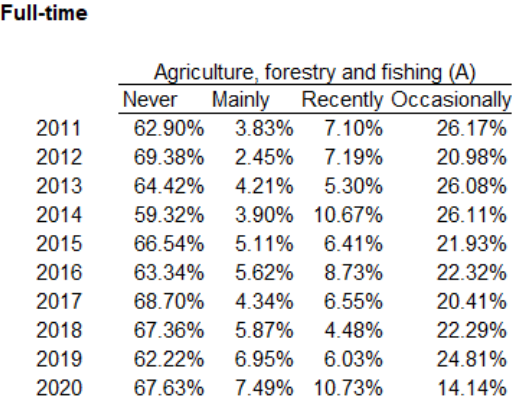
\includegraphics[width=200px]{exampleONSTable.png}
              \caption{An example data table from the ONS data. The 2019 data was extracted as it was the most recent, and converted into Python format for easy usage. See DataONS.py in the appendix.}
              \label{fig:ONSTable}
            \end{figure}
            
            The model created relies on technical computing through the use of object oriented programming to represent a person. We made this choice because it is easy and computationally cheap to spin up new instances of an OOP object, meaning it would work well when the model is reused in Part III for the Monte Carlo simulation.
            \\ \\
            The model works in the following way:
            \begin{enumerate}
                \item Determine the overall proportion of people actually working from home pre-pandemic, and call this the baseRate.
                \item For each of the persons's characteristics, such as their ethnicity, whether they work full time or part time etc we use ONS data to determine the percentage of people working from home within these categories.
                \item We then divide these by the base rate so that if a particular industry is "bang average", no change is made to the probability of working from home pre-pandemic, whereas if a given industry is more or less prone to working from home we multiply the baseRate probability by the factor industry rate over baseRate, for example.
                \item This process of multiplying the rate is repeated for each of a given person's characteristics.
                \item We then incorporate the continuous (non categoric) factors affecting working from home of commute distance and age. To incoporate commute distance we take the tanh of the commute distance in km and multiply it by the current probability of working from home for the person. This is justified because tanh goes through the origin, which means that if a person has 0 commute distance their chance of working from home becomes 0 because it is no extra effort to go into the office. As the person gets further away from the office (commute lengthens) the probability of working from home increases as they will not want to have to commute. We use tanh because it peaks at 1 meaning we can't increase the probability of working from home above 1, and once a worker gets far from their office an increase of 1km has less effect.
                \item To incorporate the age of the worker we again multiply the current probability by a new value, which in this case is defined as multiplying factor = $1.5-0.5 \cdot e^{\frac{A-20}{80}$. This yields the desired behaviour of a steady decline in likelihood of WFH with age; starting at 1 for a 20 year old due to level of tech saviness. 
            \end{enumerate}
            
        \subsection{Applying & Evaluating the Model (Results)}  
            % Considering any situations given to us in the question
            % And if none are given, make up some input data into the Model
            To evaluate the model we consider some example people. It's impossible to try all of the many intersections of the different factors but we think the following demonstrates a range of logical behaviours. The model's successful integration into Part III leading to reasonable results suggests it is good. See that section for more details.
            \begin{figure}[H] 
              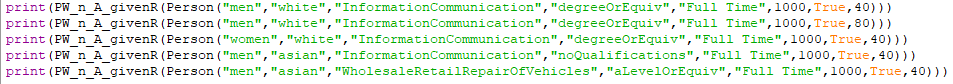
\includegraphics[width=200px]{testValues.png}
              \caption{Input to the model to apply and evaluate it}
              \label{fig:testValues}
            \end{figure}  
            \begin{figure}[H]
              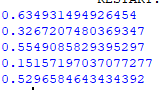
\includegraphics[width=200px]{testValuesOut.png}
              \caption{Probabilities of the respective people working from home.}
              \label{fig:testValuesOut}
            \end{figure}  
            
            